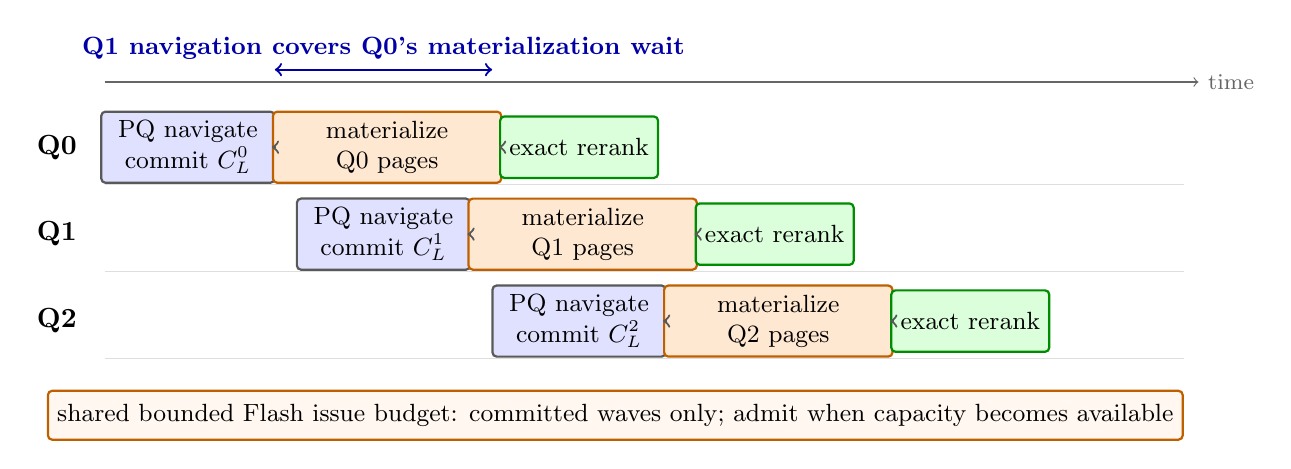
\begin{tikzpicture}[
  x=0.92cm,y=0.92cm,
  font=\small,
  lane/.style={font=\bfseries,anchor=east},
  stage/.style={draw=black!65,thick,rounded corners=1.5pt,
                minimum height=0.78cm,align=center,font=\small},
  nav/.style={stage,fill=blue!12},
  materialize/.style={stage,fill=orange!18,draw=orange!75!black},
  rank/.style={stage,fill=green!14,draw=green!55!black},
  flow/.style={->,thick,draw=black!65}
]
  \draw[->,black!60] (1.20,4.95)--(16.30,4.95)
    node[anchor=west,font=\footnotesize] {time};
  \node[font=\small\bfseries,blue!65!black] at (5.05,5.42)
    {Q1 navigation covers Q0's materialization wait};
  \draw[<->,thick,blue!65!black] (3.55,5.12)--(6.55,5.12);

  \node[lane] at (0.95,4.05) {Q0};
  \node[lane] at (0.95,2.85) {Q1};
  \node[lane] at (0.95,1.65) {Q2};
  \foreach \y in {4.05,2.85,1.65}
    \draw[black!13] (1.20,\y-0.52)--(16.10,\y-0.52);

  \node[nav,minimum width=2.20cm] (q0n) at (2.35,4.05)
    {PQ navigate\\commit $C_L^0$};
  \node[materialize,minimum width=2.90cm] (q0m) at (5.10,4.05)
    {materialize\\Q0 pages};
  \node[rank,minimum width=2.00cm] (q0r) at (7.75,4.05)
    {exact rerank};
  \draw[flow] (q0n)--(q0m); \draw[flow] (q0m)--(q0r);

  \node[nav,minimum width=2.20cm] (q1n) at (5.05,2.85)
    {PQ navigate\\commit $C_L^1$};
  \node[materialize,minimum width=2.90cm] (q1m) at (7.80,2.85)
    {materialize\\Q1 pages};
  \node[rank,minimum width=2.00cm] (q1r) at (10.45,2.85)
    {exact rerank};
  \draw[flow] (q1n)--(q1m); \draw[flow] (q1m)--(q1r);

  \node[nav,minimum width=2.20cm] (q2n) at (7.75,1.65)
    {PQ navigate\\commit $C_L^2$};
  \node[materialize,minimum width=2.90cm] (q2m) at (10.50,1.65)
    {materialize\\Q2 pages};
  \node[rank,minimum width=2.00cm] (q2r) at (13.15,1.65)
    {exact rerank};
  \draw[flow] (q2n)--(q2m); \draw[flow] (q2m)--(q2r);

  \node[draw=orange!75!black,thick,rounded corners=1.5pt,fill=orange!6,
        minimum width=11.9cm,minimum height=0.62cm,font=\small]
    at (8.25,0.35)
    {shared bounded Flash issue budget: committed waves only; admit when capacity becomes available};
\end{tikzpicture}
